\section{Design and Implementation}
\subsection{Approach}
The purpose of a network visualiser is to allow users to analyse and get insight into how they use the network\cite{Ruan2018}. It also allows network managers(advanced users) and researchers to schedule and perform measurements. The results of the measurements are also displayed on interactive graphs for further analysis.
\paragraph{}
For this project an iterative user-centred design(UCD) approach was adopted. This entails that the user is involved throughout the whole design process so that the visualisation produced meets every need that the user has\cite{Andrews:2006:EIV:1168149.1168151}. The goal of this approach is to find out the needs and tasks of the user and then design based on that\cite{Dylggduu}. This visualisation platform is developed for a system that is to be deployed at a local community network called iNethi in Cape Town. Users of this visualisation platform are expected to be network researchers, network managers and general users of the network.
\paragraph{}
This approach consisted of three phases:early envisioning phase, the global specification phase and the detailed specification phase\cite{Kulykinbook}.
\paragraph{}
The early envisioning phase entails the analysis of the users, the environment they are in and their tasks. This will enable us to profile users and gather requirements in the process\cite{Kulykinbook}. In the context of a network visualiser, the would mean understanding the type of data that user would to see visualised and analyse. A number of methods can be employed to obtain this which include surveys, interviews and focus groups\cite{Kulykinbook} \cite{Abras04user-centereddesign}.
\paragraph{}
In the global specification phase and the detailed phase, a designer comes up with a solution and presents it to users\cite{Abras04user-centereddesign} \cite{Kulykinbook}. Each phase may contain multiple iterations of design and analysis with evaluations taking place in all phases\cite{Abras04user-centereddesign}.
\paragraph{}
\begin{figure}[b]
	\centering
	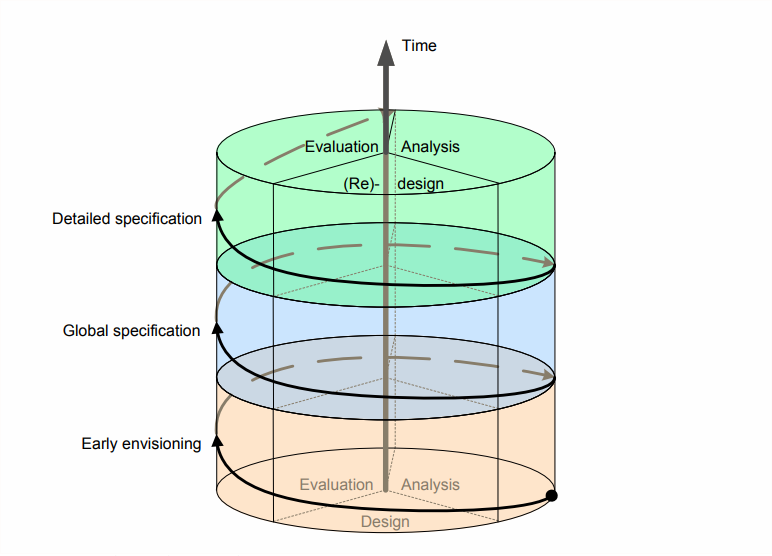
\includegraphics[width=0.7\linewidth]{images/img1}
	\caption{User-centered visualisation design process\cite{Abras04user-centereddesign}}
	\label{fig:img1}
\end{figure}

\paragraph{}
Users generally have different abilities and tasks to perform on the visualisation tool. Due to these differences it is imperative that a detailed analysis of the users, their environment and their tasks is performed before the design of the visualisation platform.

\subsection{Early envisioning}
The first iteration of the design process was early envisioning. At this iteration the main goal was to understand potential users(nature of the users) and have a clear understanding of the tasks they perform and the environment in which they perform the tasks in\cite{Valiati:2006:TTG:1168149.1168169}. The information gathered here is used to command the design of the visualisation and its functionality.

\subsubsection{Requirements Gathering}
To gather the needed information, the team attended a meeting where issues concerning the iNethi network were to be discussed. The meeting also consisted of Ocean View community members, University Of Cape Town(UCT) networking researchers,UCT professors and other technical staff. Some of the stakeholders in the meeting were members of the UCT Information and Communications Technologies for Development(ICT4D). In this meeting the use cases of the project were outlined to potential users and various stakeholders.
\paragraph{}
Specific questions concerning the network and relevance of the project were answered by stakeholders. The team also gained understanding of the nature of potential users and the environment in which the visualisation tool will be used. Some potential users also suggested features for the visualisation that would be useful to any other users. The feedback obtained ensured that the visualisation design would meet the needs of potential users and stakeholders.

\subsubsection{Implementation}
After the meeting with stakeholders and potential users, the team set out to develop a prototype of the visualisation. An interactive prototype was created using adobe xd. The prototype was limited in functionality but allowed the user to navigate from one page to another while performing different operations.The prototype did not use any real world data, the goal was mainly to focus on the user interface design.
\paragraph{}
Ben Shneiderman's golden rules of design were adopted and closely followed while designing the prototype. To strive for consistency, a blue and white theme was adopted and used in all the pages of the application. Visuals were also used to reduce short-term memory while using the application. The image on figure 2 shows the prototype screens and how the user would navigate from one to the next.


\begin{figure*}
	\centering
	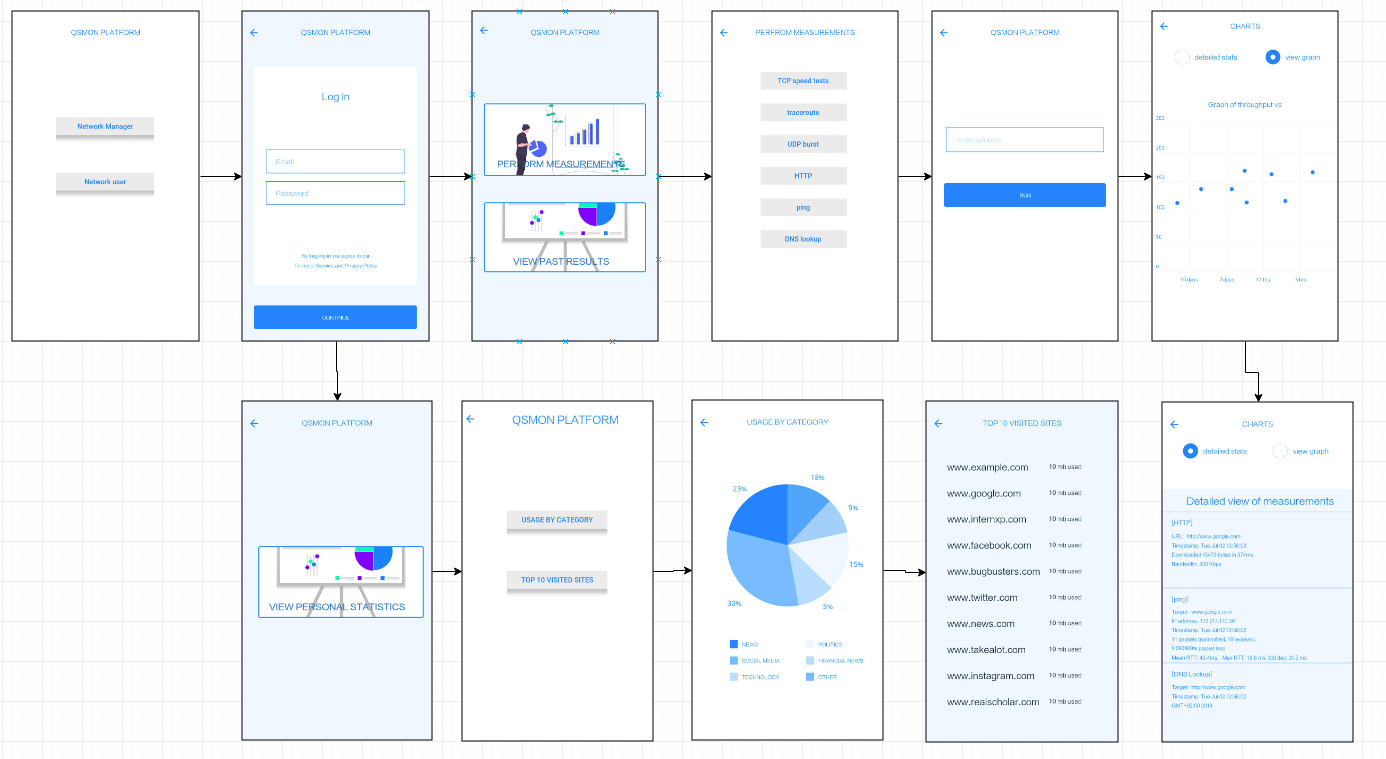
\includegraphics[width=1\linewidth]{images/proto}
	\caption{First prototype of the visualizer}
	\label{fig:proto}
\end{figure*}

\subsubsection{Evaluation}
After weeks of designing the prototype, four potential users were invited from the community of Ocean View to UCT. Amongst them were two community leaders that are involved in the running of the iNethi network. The other two were members of the community that would use the platform as end users.
\paragraph{}
A usability study which involved semi-structured interviews was carried out with potential users. Users were allowed to go through the app and encouraged to be talking and pointing out what they are doing at each stage. While this was happening the team was observing users, their facial reaction and what they are saying. At beginning of each session the user will be presented with the first page of the app and they were encouraged to navigate through the app from there on and perform different operations. To avoid bias, users did the testing of the application separately.
\paragraph{}
At the end of each session the users were asked to provide feedback in written form. Results indicated that three out of four users found the application not difficult to use and the same number said that the application would be useful to the community. On top of the that some users suggested new features which they thought would be very useful if incorporated into the application.

\subsection{Global Specification}
In this phase, solutions that have been developed are proposed and presented to users and stakeholders\cite{Kulykinbook}.
\subsubsection{Analysis and Requirements Gathering}
The feedback from the first prototype was gathered and put together for the next phase of the design approach. This feedback was to be used to command the initial design of the actual application.
\subsubsection{Implementation}
Based on the feedback gathered from the previous phase, it was decided that the development of the actual user interface be started. The user interface was designed to be a responsive web based system that the user can use comfortably on their mobile devices.
\paragraph{}
React, a JavaScript front end framework was chosen for the development of the web interface.
